%%******************************************************************************
%% Instruções para compilação e apresentação
%%******************************************************************************

% para compilar use SHIFT + ALT + E (compilar direto para PDF)
%
% para apresentação use o adobe para evitar o flicker
%


\documentclass{beamer}


% ===============================================================
% compilar com XeLaTeX (Shift+Alt+E no WinEdt) em PORTUGUES
%\XeTeXinputencoding latin1
% ===============================================================



%%******************************************************************************
%% PACKAGES
%%******************************************************************************
\usepackage{beamerthemesplit}
\usepackage{beamerfoils}
\usepackage[T1]{fontenc}
\usepackage[latin1,utf8]{inputenc}
\usepackage[english,brazil]{babel}
\usepackage{indentfirst}         % indentacao de primeiro paragrafo
\usepackage{subfigure}
%\usepackage{subfig}
\usepackage{epsfig}
\usepackage{cite}
\usepackage{setspace}
\usepackage{rotating}
\usepackage{graphicx}
\usepackage{dsfont}
\usepackage{enumerate}
\usepackage{amsmath}
\usepackage{color}
\usepackage{bbm}
\usepackage{amssymb}
\usepackage{ulem}
\usepackage{comment}
\usepackage{glossaries}
\usepackage{pdflscape}
\usepackage{adjustbox}
\usepackage{tikz}
\usepackage{ragged2e}
\usepackage{gensymb}

\newcommand*\circled[1]{\tikz[baseline=(char.base)]{ \scriptsize
            \node[shape=circle,draw,inner sep=0.5pt] (char) {#1};}}



\mode<presentation>{

    %%******************************************************************************
    %% Temas e Cores
    %%******************************************************************************
    %%
    %% Temas
    %\usetheme{Berkeley}    % left bar
    %\usetheme{Antibes}     % tree header
    %\usetheme{Boadilla}     % BEST ----- very plain
    %\usetheme{Warsaw}
    %\usetheme{Rochester}
    %\usetheme{Madrid}
    %\usetheme{Goettingen}  % bad ---- right bar
    %\usetheme{Ilmenau}
    \usetheme{CambridgeUS} % good with dolphin
    %%
    %% Cores
    %\usecolortheme{whale}
    \usecolortheme{dolphin}
    %******************************************************************************




    %%******************************************************************************
    %% Setar a caixa de navegação
    %%******************************************************************************
    \usefonttheme[onlymath]{serif}
    %um dos dois abaixo
    \newcommand{\currentframe}{\hspace{2.3cm}\insertframenumber}%/\inserttotalframenumber}
    %\setbeamertemplate{footline}[page number]

    \setbeamertemplate{navigation symbols}{}
    \AtBeginSection[]
    {
    %\begin{frame}
    %\frametitle{Sumário}
    %\tableofcontents[currentsection,hideallsubsections]
    %\end{frame}
    }
    
    %\usepackage{beamerouterthemeshadow}
    %\usepackage{beamerouterthemesmoothtree}
    %\usepackage{beamercolorthemeorchid}
    %\usepackage{beamerinnerthemerounded}
    %\setbeamercovered{transparent}
    % comment out to completely hide covered material
}% end \mode<presentation>{


%*******************************************************************************
% não sei!!
%\usefonttheme[onlylarge]{structuresmallcapsserif}
\usepackage{times}
%*******************************************************************************




%%******************************************************************************
%% PÁGINA DO TÍTULO
%%******************************************************************************

\title[Ciência de Dados]{Comparação de Métodos de Classificação de Ruído Acústico}
%\title[Short Title]{Long Title}

\author[Nascimento, Farias, Alves]
{
Antônio Nascimento, Felipe Farias e Marília Alves
%Eddie B. L. Filho, Waldir S. S. Junior  \\
%\textit{Orientador}: Prof.Dr. Waldir Sabino da Silva Junior \\
%\textit{Co-Orientador}: Prof.Dr. Eddie Batista de Lima Filho
}


\institute[IME]{%
Instituto Militar de Engenharia \\
%Universidade do Estado do Amazonas
}

\date[Agosto de 2017] % (optional, should be abbreviation of conference name)
%{Simpósio Brasileiro de Telecomunicações \\ 
{Agosto de 2017}
% - Either use conference name or its abbreviation.


%%******************************************************************************
%% CORPO PRINCIPAL
%%******************************************************************************

\begin{document}

%\MyLogo{\includegraphics[scale=0.9]{figuras/logo-lab-apresentacao.eps}}

\justifying

\begin{frame}
  \titlepage
\end{frame}


%%==============================================================================
%% SEÇÃO Sumário
%%==============================================================================

%\MyLogo{\includegraphics[scale=0.5]{figuras/logo-lab-apresentacao.eps}}

\section[Sumário]{}
\begin{frame}
  \tableofcontents
\end{frame}



%%==============================================================================
%% SEÇÕES
%%==============================================================================

\section{Introdução}

\subsection{Processamento de Sinais Acústicos em Ruído}

\begin{frame}
	\justifying
  	\frametitle{Ruído em Tarefas de PDS}
  	
  	\begin{itemize}
  		\setlength\itemsep{1em}
  		\item Tarefas de Processamento de Sinais Acústicos
        \begin{itemize}
        	\item Reconehcimento de Locutor
            \item Localização
            \item Reconhecimento de Fala
        \end{itemize}
        \item Ruído é \textbf{o principal} desafio.
        \begin{itemize}
        \item Queda de rendimento.
        \end{itemize}
  	\end{itemize}
\end{frame}

\begin{frame}
	\justifying
  	\frametitle{Estudar e Analisar Ruído}
  	\begin{itemize}
  		 \setlength\itemsep{1em}
  		\item Detecção (presença/ausência)
        \item Classificação
        \begin{itemize}
        \item Inclusão em Ferramentas de Realce
        \end{itemize}
  	\end{itemize}
\end{frame}

\subsection{Objetivos}

\begin{frame}
	\justifying
  	\frametitle{Objetivos do Trabalho}
  	
  	\begin{itemize}
  		\setlength\itemsep{1em}
  		\item Comparar desempenho de técnicas de clasificação de áudio conhecidas na literatura na tarefa de classificação de ruído.
        
 	\end{itemize}
  		
\end{frame}

\begin{frame}
	\justifying
  	\frametitle{Metodologia}
  	
  	\begin{figure}[ht]
    	\centering
		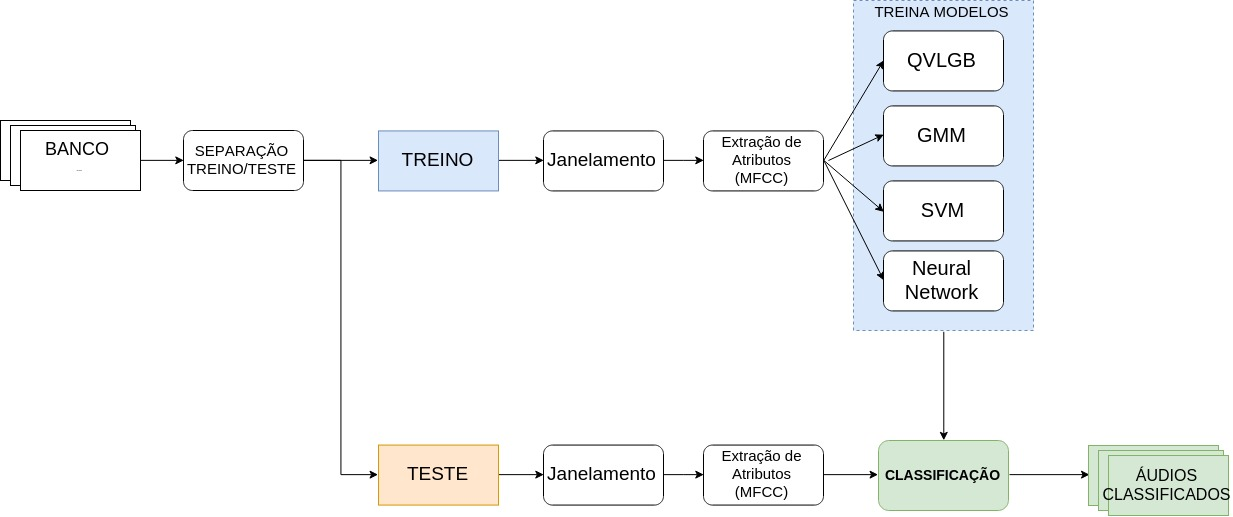
\includegraphics[width=\textwidth]{diagrama_artigo_maior.jpg}
		\caption{Diagrama da Classificação}
		\label{fig:diagclass}
	\end{figure}

  		
\end{frame}

\section{Técnicas Utilizadas}

\begin{frame}
    \frametitle{A base de dados NOISEX-92}
    
    \begin{itemize}
    	\setlength\itemsep{1em}
        \item 15 classes
    	\item Formato .wav
        \item Tamanho: 3m55s
	\end{itemize}
    
    \begin{table}[ht]
	\centering
	\caption{Classes na base de dados NOISEX.}
	\label{tab:noisex}
	\resizebox{\textwidth}{!}{\begin{tabular}{lllll}
		\hline
		Babble & Buccaneer 1 & Buccaneer 2 & Destroyer Engine & Destroyer Operations Room\\
		F16 & Factory Floor 1 & Factory Floor 2 & HF Channel & Leopard\\
		M109 & Machine Gun & Pink Noise & Volvo & White Noise\\
		\hline
	\end{tabular}}
\end{table}
    
    
\end{frame}

\subsection{Validação Cruzada}

\begin{frame}
	\frametitle{Validação Cruzada}
	
	\begin{figure}[ht]
    	\centering
		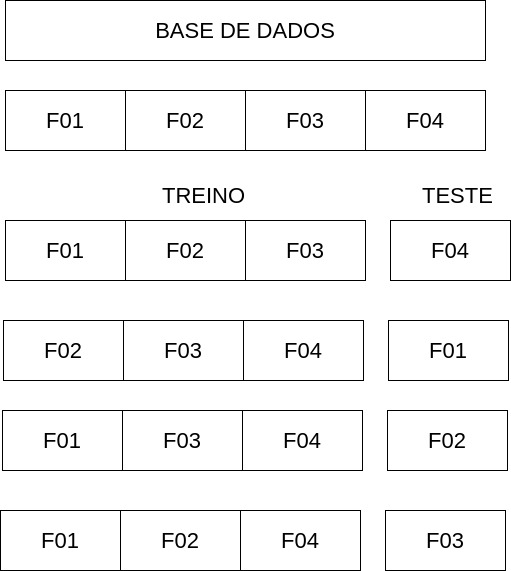
\includegraphics[width=.4\textwidth]{crossvalid.jpg}
		\caption{Diagrama da Classificação}
		\label{fig:diagclass}
	\end{figure}
    
\end{frame}


\subsection{Extração de Atributos do Áudio}
  		
%\begin{frame}
%  	\frametitle{LPC}
%  	\begin{itemize}
%  		\setlength\itemsep{1em}
%  		\item VAI QUE É TUA MARILIA
%  		\item LPC
%  	\end{itemize}
%\end{frame}


\begin{frame}
  	\frametitle{Mel-Frequency Cepstral Coefficient (MFCC)}
  	%\begin{itemize}
  	%	\setlength\itemsep{1em}
  	%	\item Coeficientes Mel-Cepstrais
  	%	\begin{itemize}
  	%		\item porque é melhor?
  	%	\end{itemize}
  	%\end{itemize}
    
    \begin{figure}[ht]
    \centering
	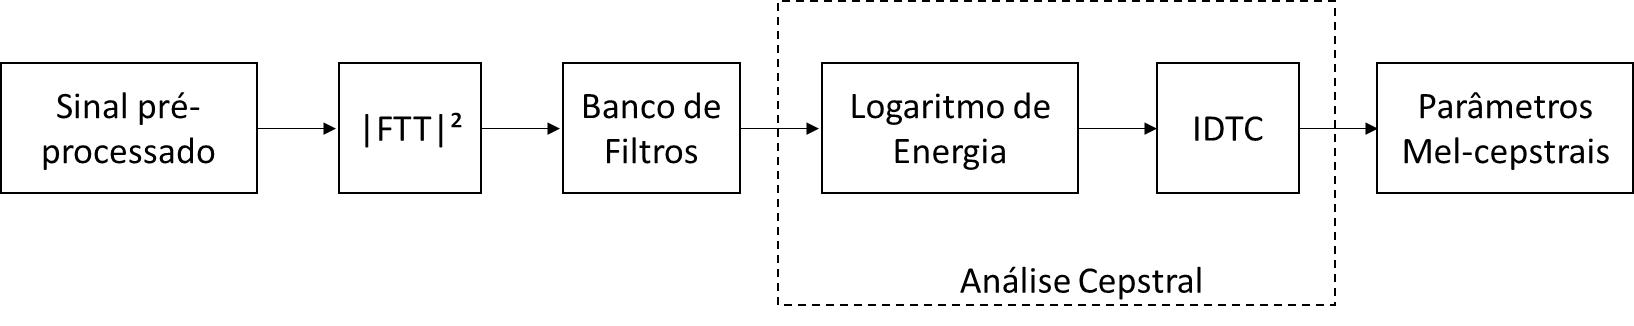
\includegraphics[width=\textwidth]{mfcc.jpg}
	\caption{Extração do MFCC}
	\label{fig:exampleFig1}
	\end{figure}
\end{frame}

\section{Experimentos}



\subsection{Condições Iniciais}

\begin{frame}
	\frametitle{Condições Iniciais}
	
    \begin{itemize}
    	\setlength\itemsep{1em}
    	\item Entrada dos classificadores:
        \begin{itemize}
    	    \item 15 classes;
            \item 275370 amostras;
            \item 39 coeficientes;
        \end{itemize}
    	
        \item Ferramentas Utilizadas:
        \begin{itemize}
			\item MATLAB;
        	\begin{itemize}
        		\item toolbox Neural Network;
        		\item toolbox SVM;
        	\end{itemize}
        	\item Voicebox;
		\end{itemize}
	\end{itemize}
\end{frame}




\subsection{Métodos Utilizados}


\begin{frame}

	\frametitle{QV LGB (intro)}
	
	\begin{itemize}	
		\item detalhes das especificações aqui
	\end{itemize}
	
\end{frame}


\begin{frame}

	\frametitle{QV LGB (resultados)}
	
	\begin{table}[h]
\centering
\caption{Matriz de Confusão da classificação usando QVLGB}
\label{tab:confusion_qvlgb}
\resizebox{\textwidth}{!}{\begin{tabular}{l||l|l|l|l|l|l|l|l|l|l|l|l|l|l|l}
\hline
& Babble & Bucc 1 & Bucc 2 & Dest Eng & Dest Ops & F16 & Fac 1 & Fac 2 & HFChn & Leop & M109 & MachGun & Pink & Volvo & White \\
\hline
\hline
Babble & 6,5\% & & & & & & 0,1\% & 0,1\% & & & & & & & \\
\hline
Buccaneer 1 & &6,6\% & & & & & & & & & & & & & \\
\hline
Buccaneer 2  & & & 6,7\% & & & & & & & & & & & & \\
\hline
Destroyer Engine  & & & & 6,6\% & & & & & & & & & & & \\
\hline
Destroyer Ops & & & & & 6,5\%& & & & & & & & & & \\
\hline
F16 & & & & & & 6,6\% & & & & & & & & & \\
\hline
Factory 1 & & & & & & & 6,0\% &0,2\% & & & & & 0,1\% & & \\
\hline
Factory 2 & & & & & & & 0,3\%& 6,4\% & & & & & & & \\
\hline
HF Channel & & & & & & & & & 6,7\% & & & & & & \\
\hline
Leopard & & & & & & & & & &6,6\% & & & & & \\
\hline
M109 & & & & & & & & & & &6,6\% & & & & \\
\hline
Machine Gun & & & & & & & & & & & &6,6\% & & & \\
\hline
Pink & & & & & & & 0,2\% & & & & & &6,6\% & & \\
\hline
Volvo & & & & & & & & & & & & & &6,6\% & \\
\hline
White & & & & & & & & & & & & & & & 6,7\%\\
\hline
\end{tabular}}
\end{table}
	
\end{frame}


\begin{frame}

	\frametitle{Gaussian Mixture Model (intro)}
	
	\begin{itemize}	
		\item introdução bonitinha aqui
	\end{itemize}
	
\end{frame}





\begin{frame}

	\frametitle{Gaussian Mixture Model (resultados)}
	
	\begin{table}[h]
\centering
\caption{Matriz de Confusão da classificação usando GMM}
\label{tab:confusion_gmm}
\resizebox{\textwidth}{!}{\begin{tabular}{l||l|l|l|l|l|l|l|l|l|l|l|l|l|l|l}
\hline
& Babble & Bucc 1 & Bucc 2 & Dest Eng & Dest Ops & F16 & Fac 1 & Fac 2 & HFChn & Leop & M109 & MachGun & Pink & Volvo & White \\
\hline
\hline
Babble & 6,5\% & & & & & & 0,1\% & 0,1\% & & & & & & & \\
\hline
Buccaneer 1 & &6,6\% & & & & & & & & & & & & & \\
\hline
Buccaneer 2  & & & 6,7\% & & & & & & & & & & & & \\
\hline
Destroyer Engine  & & & & 6,6\% & & & & & & & & & & & \\
\hline
Destroyer Ops & & & & & 6,5\%& & & & & & & & & & \\
\hline
F16 & & & & & & 6,6\% & & & & & & & & & \\
\hline
Factory 1 & & & & & & & 6,0\% &0,2\% & & & & & 0,1\% & & \\
\hline
Factory 2 & & & & & & & 0,3\%& 6,4\% & & & & & & & \\
\hline
HF Channel & & & & & & & & & 6,7\% & & & & & & \\
\hline
Leopard & & & & & & & & & &6,6\% & & & & & \\
\hline
M109 & & & & & & & & & & &6,6\% & & & & \\
\hline
Machine Gun & & & & & & & & & & & &6,6\% & & & \\
\hline
Pink & & & & & & & 0,2\% & & & & & &6,6\% & & \\
\hline
Volvo & & & & & & & & & & & & & &6,6\% & \\
\hline
White & & & & & & & & & & & & & & & 6,7\%\\
\hline
\end{tabular}}
\end{table}
	
\end{frame}


\begin{frame}

	\frametitle{Neural Network  (intro)}
	
	\begin{itemize}	
		\item introdução bonitinha aqui
	\end{itemize}
	
\end{frame}





\begin{frame}

	\frametitle{Neural Network (resultados)}
	
	\begin{table}[h]
\centering
\caption{Matriz de Confusão da classificação usando Neural Network}
\label{tab:confusion_nn}
\resizebox{\textwidth}{!}{\begin{tabular}{l||l|l|l|l|l|l|l|l|l|l|l|l|l|l|l}
\hline
& Babble & Bucc 1 & Bucc 2 & Dest Eng & Dest Ops & F16 & Fac 1 & Fac 2 & HFChn & Leop & M109 & MachGun & Pink & Volvo & White \\
\hline
\hline
Babble & 6,5\% & & & & & & 0,1\% & 0,1\% & & & & & & & \\
\hline
Buccaneer 1 & &6,6\% & & & & & & & & & & & & & \\
\hline
Buccaneer 2  & & & 6,7\% & & & & & & & & & & & & \\
\hline
Destroyer Engine  & & & & 6,6\% & & & & & & & & & & & \\
\hline
Destroyer Ops & & & & & 6,5\%& & & & & & & & & & \\
\hline
F16 & & & & & & 6,6\% & & & & & & & & & \\
\hline
Factory 1 & & & & & & & 6,0\% &0,2\% & & & & & 0,1\% & & \\
\hline
Factory 2 & & & & & & & 0,3\%& 6,4\% & & & & & & & \\
\hline
HF Channel & & & & & & & & & 6,7\% & & & & & & \\
\hline
Leopard & & & & & & & & & &6,6\% & & & & & \\
\hline
M109 & & & & & & & & & & &6,6\% & & & & \\
\hline
Machine Gun & & & & & & & & & & & &6,6\% & & & \\
\hline
Pink & & & & & & & 0,2\% & & & & & &6,6\% & & \\
\hline
Volvo & & & & & & & & & & & & & &6,6\% & \\
\hline
White & & & & & & & & & & & & & & & 6,7\%\\
\hline
\end{tabular}}
\end{table}
	
\end{frame}


\begin{frame}

	\frametitle{Support Vector Machines (intro)}
	
	\begin{itemize}	
		\item introdução bonitinha aqui
	\end{itemize}
	
\end{frame}





\begin{frame}

	\frametitle{Support Vector Machines  (resultados)}
	
	\begin{table}[h]
\centering
\caption{Matriz de Confusão da classificação usando SVM}
\label{tab:confusion_svm}
\resizebox{\textwidth}{!}{\begin{tabular}{l||l|l|l|l|l|l|l|l|l|l|l|l|l|l|l}
\hline
& Babble & Bucc 1 & Bucc 2 & Dest Eng & Dest Ops & F16 & Fac 1 & Fac 2 & HFChn & Leop & M109 & MachGun & Pink & Volvo & White \\
\hline
\hline
Babble & 6,5\% & & & & & & 0,1\% & 0,1\% & & & & & & & \\
\hline
Buccaneer 1 & &6,6\% & & & & & & & & & & & & & \\
\hline
Buccaneer 2  & & & 6,7\% & & & & & & & & & & & & \\
\hline
Destroyer Engine  & & & & 6,6\% & & & & & & & & & & & \\
\hline
Destroyer Ops & & & & & 6,5\%& & & & & & & & & & \\
\hline
F16 & & & & & & 6,6\% & & & & & & & & & \\
\hline
Factory 1 & & & & & & & 6,0\% &0,2\% & & & & & 0,1\% & & \\
\hline
Factory 2 & & & & & & & 0,3\%& 6,4\% & & & & & & & \\
\hline
HF Channel & & & & & & & & & 6,7\% & & & & & & \\
\hline
Leopard & & & & & & & & & &6,6\% & & & & & \\
\hline
M109 & & & & & & & & & & &6,6\% & & & & \\
\hline
Machine Gun & & & & & & & & & & & &6,6\% & & & \\
\hline
Pink & & & & & & & 0,2\% & & & & & &6,6\% & & \\
\hline
Volvo & & & & & & & & & & & & & &6,6\% & \\
\hline
White & & & & & & & & & & & & & & & 6,7\%\\
\hline
\end{tabular}}
\end{table}
	
\end{frame}

\begin{frame}

	\frametitle{Comparação}
	
	\begin{table}[ht]
\centering
\caption{Accuracy per class for the methods compared.}
\label{tab:acc}
\resizebox{.7\textwidth}{!}{\begin{tabular}{l|llll}
\hline
Class & QV LGB & GMM & Neural Network & SVM \\
\hline
Babble & 88,2\% & 98,9\% & 97,5\% &  \\
Bucanneer 1 & 96,6\% & 99,1\% & 99,1\% & \\
Bucanneer 2 & 98,8\% & 99,7\% & 99,8\% & \\
Destroyer Engine & 99,8\% & 99,7\% & 99,7\% & \\
Destroyer Ops & 90,8\% & 96,9\% & 98,3\% &\\
F16 & 95,2\% & 99,10\% & 97,6\% &\\
Factory 1 & 59,3\% & 87,6\% & 92,3\% &\\
Factory 2 & 93,9\% & 95,0\% & 94,7\% &\\
HF Channel & 100,0\% & 100,0\% & 99,9\% &\\
Leopard & 99,1\% & 99,6\% & 99,4\% &\\
M109 & 94,1\% & 99,3\% & 99,3\% &\\
Machine Gun & 7,1\% & 99,5\% & 99,5\% &\\
Pink & 99,7\% & 98,0\% & 96,9\% &\\
Volvo & 90,8\% & 99,4\% & 99,7\% &\\
White & 99,9\% & 99,9\% & 100,0\% &\\
\hline
\textbf{OVERALL} & 89,2\% & 98,0\% & 98,4\% & \\
\hline
\end{tabular}}
\end{table}
	
\end{frame}

\section{Considerações Finais}

\begin{frame}

	\frametitle{Conclusões}
	
	\begin{itemize}
		\setlength\itemsep{1em}
		
		\item Concluímos que o trabalho foi muito trabalhoso.
	
	\end{itemize}


\end{frame}

\begin{frame}

	\frametitle{Trabalhos Futuros}
	
	\begin{itemize}
		\setlength\itemsep{1em}
		
		\item Estender a comparação a outros métodos de classificação;
        \item Aumentar a diversidade da base de dados;
		\item Investigar desempenho de comitê de classificação;
        \item Investigar técnicas de Deep Learning.
	
	\end{itemize}


\end{frame}


\begin{frame}
	\frametitle{Obrigado!}
    
    \centering
    
    \begin{itemize}
    	\setlength\itemsep{2em}
		\item Obrigado pela atenção!
	\end{itemize}

\end{frame}

\end{document}
